
\documentclass[10pt,landscape]{scrartcl}

\usepackage[english]{babel}
% \usepackage[ngerman]{babel}
\usepackage[utf8]{inputenc}

\usepackage{lmodern}

\usepackage{ifthen}

\usepackage{graphicx}
% \usepackage{pstricks}
% \usepackage{relsize}
% \usepackage[decimalsymbol=comma,exponent-product = \cdot, per=frac]{siunitx}
% \sisetup{range-phrase=\,bis\,}

\usepackage{xargs}
\usepackage{calc}
\usepackage{amsmath}
\usepackage{amsfonts}
\usepackage{mathtools}
\usepackage{amssymb}

\usepackage{cancel}
\usepackage{trfsigns}
\usepackage{array}
\usepackage{enumerate}
\usepackage{enumitem}

\usepackage{caption}
\usepackage{subcaption}

\usepackage{multicol}

\usepackage{pdflscape}
\usepackage[table]{xcolor}

\usepackage{float}

%%%%%%%%%%%%%%%%%%%%%%%%%%%%%%%%%%%%%%%%%%%%%%%%%%%%%%%%%%%%%%%%%%%%%%%%%%%%%%%%
\newboolean{WITHPSTRICKS}
\setboolean{WITHPSTRICKS}{false}


\newcommand{\PROFESSOR}{Prof.\ Dr.\ Thomas Carraro}
\newcommand{\ASSISTANT}{\setlength{\tabcolsep}{0pt}\begin{tabular}{l} Dr. Ulrike Kochan-Eilers\end{tabular}}

\newcommand{\Jahr}{2025}
% \newcommand{\Trimester}{HT}
\newcommand{\Trimester}{WT}
\newcommand{\Kurs}{Mathematik II/B (WI/ET)}
\newcommand{\TYPE}{Aufgabenblatt}
\newcommand{\BLATT}{5}
\newcommand{\TOPIC}{L'Hospital, Optimierungsproblem, Kurvendiskussion, Monotonieverhalten}

%%%%%%%%%%%%%%%%%%%%%%%%%%%%%%%%%%%%%%%%%%%%%%%%%%%%%%%%%%%%%%%%%%%%%%%%%%%%%%%%
\newboolean{mitLoes}
\setboolean{mitLoes}{false}
\setboolean{mitLoes}{true}

%%%%%%%%%%%%%%%%%%%%%%%%%%%%%%%%%%%%%%%%%%%%%%%%%%%%%%%%%%%%%%%%%%%%%%%%%%%%%%%%


%\setboolean{WITHPSTRICKS}{false}
\setboolean{WITHPSTRICKS}{true}


\usepackage{tikz}
\usetikzlibrary{arrows,automata,backgrounds,calendar,decorations.pathmorphing,fadings,shadings,calc,intersections}
\usetikzlibrary{decorations.pathreplacing}
\usetikzlibrary{decorations.shapes}
\usetikzlibrary{decorations.footprints}
\usetikzlibrary{decorations.text}
\usetikzlibrary{positioning}
\usetikzlibrary{through}
\usepackage[utf8]{inputenc}


\ifthenelse{\boolean{WITHPSTRICKS}}{%
\usepackage{auto-pst-pdf}
\usepackage{pstricks,pst-plot,pst-text}
}{}

\usepackage{pgfplots}

%%%%%%%%%%%%%%%%%%%%%%%%%%%%%%%%%%%%%%%%%%%%%%%%%%%%%%%%%%%%%%%%%%%%%%%%%%%%%%%%
\usepackage{mbdefAufgaben}

%%%%%%%%%%%%%%%%%%%%%%%%%%%%%%%%%%%%%%%%%%%%%%%%%%%%%%%%%%%%%%%%%%%%%%%%%%%%%%%%
\newboolean{mitErg}
%\setboolean{mitErg}{false}

%%%%%%%%%%%%%%%%%%%%%%%%%%%%%%%%%%%%%%%%%%%%%%%%%%%%%%%%%%%%%%%%%%%%%%%%%%%%%%%%
\newcounter{Aufg}
\setcounter{Aufg}{0}
\newcounter{Blatt}
\setcounter{Blatt}{1}

%%%%%%%%%%%%%%%%%%%%%%%%%%%%%%%%%%%%%%%%%%%%%%%%%%%%%%%%%%%%%%%%%%%%%%%%%%%%%%%%
%\usepackage{KopfEnglish}

% Seitenraender
%\textwidth = 285mm
%\textheight = 180mm
%\leftmargin 5mm
%\oddsidemargin = -20mm
%\evensidemargin = -20mm
%\topmargin = -25mm
%\parindent 0cm
%\columnsep 2cm

% % % Aufgabenstellung
% % % Schwierungkeitsgrad mit "e" , "f" oder "v" angeben
% % % "e" Einführung   
% % % "f" Festigung
% % % "v" Vertiefung  

\newcommand{\Aufgabe}[3][]{
\stepcounter{Aufg}
\subsubsection*{Aufgabe 
\arabic{Aufg}\ifthenelse{\equal{#1}{e}}{}{\ifthenelse{\equal{#1}{f}}{
$\!\!{}^\star$}{\ifthenelse{\equal{#1}{v}}{$^{\star\star}$}{}}}{: #2}}
{#3}
}
% % % Ergebnisse jeweils am Ende des Aufgabenblattes Anzeigen
\newcommand{\Ergebnisse}{}
\makeatletter
\newcommand{\Ergebnis}[1]{
	\g@addto@macro{\Ergebnisse}{#1}
}
\makeatother
\makeatletter
\newcommand{\ErgebnisC}[2]{
\@ifundefined{c@#1}
{\newcounter{#1}}
{}
\setcounter{#1}{\theAufg}

\ifthenelse{\boolean{mitErg}}{	\g@addto@macro{\Ergebnisse}{\subsubsection*{Ergebnisse zu Aufgabe \arabic{#1}:}
}%
	\g@addto@macro{\Ergebnisse}{#2}}{}
}
\makeatother


% % % Lösungen
\newcommand{\Loesung}[1]{
	\ifthenelse{\boolean{mitLoes}}
	{\subsubsection*{Lösung \arabic{Aufg}:}
		#1}
	{}
}
% % % % % % % % % % % % % % % % % % % % % % % % % % % % % % % % % % % % % % % % % % % % % % % % % % % % % %
% % % % % % % % % % % % % % % % % % % % % % % % % % % % % % % % % % % % % % % % % % % % % % % % % % % % % %
% % % % % % % % % % % % % % % % % % % % % % % % % % % % % % % % % % % % % % % % % % % % % % % % % % % % % %
\begin{document}
%\begin{twocolumn}
% % % % % % % % % % % % % % % % % % % % % % % % % % %

%%%%%%%%%%%%%%%%%%%%%%%%%%%%%%%%%%%%%%%%%%%%%%%%%%%%%%%%%%%%%%%%%%%%%%%%%%%%%%%%
% Set the TITLE of the sheet here:
%\uebheader{\Kurs}{\arabic{Blatt}}{\Trimester\,\Jahr}{\TOPIC}
%\uebheader{\Kurs}{\arabic{Blatt}}{\Trimester\,\Jahr}{\TOPIC}
%\uebheader{\Kurs}{\arabic{Blatt}}{\Trimester\,\Jahr}{\TOPIC}
%\ruleBig

\setboolean{mitErg}{false}
%\setboolean{mitErg}{true}


%%%%%%%%%%%%%%%%%%%%%%%%%%%%%%%%%%%%%%%%%%%%%%%%%%%%%%%%%%%%%%%%%%%%%%%%%%%%%%%%
% Set the INTRODUCTION section of the sheet here:
% \input{introduction.tex}

\textbf{Einführende Bemerkungen}

\begin{itemize}
\item Vermeiden Sie die Verwendung von Taschenrechnern oder Online-Ressourcen.
% \item Die mit einem Stern *) markierten (Teil-)Aufgaben entfallen in diesem Trimester. Stattdessen werden einzelne Online-Aufgaben im ILIAS-Kurs kenntlich gemacht, zu denen Sie dort Ihre L\"osungswege zur Korrektur hochladen k\"onnen. 
% \item Die mit zwei Sternen  **) markierten (Teil-)Aufgaben richten sich an Studierende, die die \"ubrigen Aufgaben bereits gel\"ost haben und die Inhalte weiter vertiefen m\"ochten. 
\end{itemize}

\ruleBig

%Mathe V Blatt 

\Aufgabe[e]{Regel von L'Hospital}{
Berechnen Sie mit Hilfe der Regel von L'Hospital die Grenzwerte
\begin{tabbing}
\hspace*{1em} \= a) $ \ \underset{x\to 0}\lim \dfrac{x^2 \sin x}{\tan x-x}$\,,
\hspace*{8em} \= b) 
    $\underset{x\rightarrow 0}\lim \dfrac{\ln(\EH{x}-x)}{\ln(\cos x)}$\,, \\[1ex]
\> c) $\underset{x\rightarrow \infty}\lim x(2\arctan x - \pi)$\,,
\> d) $\underset{x\rightarrow 1}\lim \dfrac{x^2-1}{x^{x}-1}$\,. 
\end{tabbing}

}

\Loesung{
\begin{abc}
\item Da sowohl Z\"ahler, als auch Nenner gegen Null konvergieren
$$\underset{x\to 0}\lim (x^2\sin x)=0=\underset{x\to 0}\lim (\tan x - x),$$
darf der Satz von L'Hospital angewendet werden: 
\begin{align*}
\underset{x\to 0}\lim \frac{x^2 \sin x}{\tan x-x} =& \underset{x\to 0}\lim \frac{2x\sin x + x^2\cos
x}{\frac 1{\cos^2 x}-1} = \underset{x\to 0}\lim \frac{2x \sin x \cos^2 x + x^2\cos^3 x}{1-\cos^2
x}\\
=&\underset{x\to 0}\lim \frac{2\sin x + 2x\cos x + 2x \cos x - x^2\sin x}{2(\cos x)^{-3}\sin x}\\
&\qquad\text{ (Erneut gehen Z\"ahler und Nenner gegen 0)}\\
=& \underset{x\to 0}\lim \frac{2\cos x + 4\cos x -4x\sin x -2x\sin x -x^2\cos x}{6(\cos
x)^{-4}\sin^2 x + 2(\cos x)^{-2}}
\end{align*}
Der Z\"ahler dieses Bruches geht gegen $6$, der Nenner gegen $2$, also ist insgesamt
$$\underset{x\to 0}\lim \frac{x^2\sin x}{\tan x-x} = \frac 6 2 =3$$

\item Auch hier kann die Regel von L'Hospital angewendet werden, da Z\"ahler und Nenner gegen Null gehen:
\begin{align*}
\lim_{x \to 0} \frac{\ln(\EH{x}-x)}{\ln(\cos x)}=& \lim_{x \to 0} \frac{\frac{\EH{x}-1}{\EH{x} - x}
}{\frac{-\sin x}{\cos x}}\\
=&\lim_{x\to 0} \frac{\EH{x} \cos x - \cos x}{-\EH{x} \sin x + x \sin x }\\
&\qquad\text{ (Erneut gehen Z\"ahler und Nenner gegen 0)}\\
=&\lim_{x\to 0} \frac{\EH{x} \cos x -\EH{x} \sin x + \sin x}{-\EH{x} \sin x - \EH{x} \cos x + \sin x +
x\cos x}=\frac 1 {-1}=-1
\end{align*}

\item Das Produkt $x(2\arctan x - \pi)$ kann in einen Quotienten umgeformt werden, dessen Z\"ahler
und Nenner jeweils gegen Unendlich gehen, danach kann die Regel von L'Hospital angewendet werden: 
\begin{align*}
 \lim\limits_{x \to \infty} x(2\arctan x - \pi)
  =& \lim\limits_{x \to \infty} \frac{2\arctan x - \pi}{x^{-1}}
  = \lim\limits_{x \to \infty} \frac{\dfrac{2}{1+x^2}}{-x^{-2}}\\
  =& -\lim\limits_{x \to \infty} \frac{2x^2}{1+x^2}\quad\text{(Z\"ahler und Nenner gehen gegen
  $\infty$)}\\
=& -\lim\limits_{x\to \infty} \frac{4x}{2x}=-2
\end{align*}


\item Da Z\"ahler und Nenner gegen Null konvergieren kann man die Regel von L'Hospital
  anwenden. Danach folgt mit  $x^x = \EH{x \ln x}$:
$$ \lim_{x \to 1} \dfrac{x^2-1}{x^{x}-1} 
   = \lim_{x \to 1} \dfrac{2x}{ (1+\ln x) \EH{x \ln x}} = 2\,.$$
\end{abc}
}

\ErgebnisC{AufganalysReglLhos001}
{
\textbf{a)} $3$, \textbf{b)} $-1$, \textbf{c)} $-2$, \textbf{d)} $2$
}

\ifthenelse{\boolean{mitLoes}}{\ruleBig \cleardoublepage}{}
% 69
\Aufgabe[e]{Optimierungsproblem}{
%
Ein Poster muss mit einer Gesamtfläche von $\bar A = 64000 \text{ mm}^2$ gedruckt werden. Es muss 10 mm Seitenränder und 25 mm obere und untere Ränder haben. Welche Höhe und Breite ergeben die maximale Druckfläche?
%

}


\Loesung{
%
Seien $x$ und $y$ die beiden Dimensionen des Plakats und $s$ die Seitenränder und $t$ die oberen und unteren Ränder. Die Gesamtfläche ist $\bar A = 64000 \text{ mm}^2= xy$ mm$^2$. Die gedruckte Fläche beträgt
\begin{align*}
A(x) &= (x-2s)(y-2t) \\
&= (x-2s)\left(\frac{\bar A}{x} -2t\right) \quad (\text{unter Verwendung der Nebenbedingung der Gesamtfläche})\\\
& = \bar A - \frac{2s}{x} \bar A - 2tx + 4 st \text{ mm}^2.
\end{align*}
Um die Fläche zu maximieren, suchen wir die stationären Punkte:
$$
A'(x) = 2s\bar A \frac{1}{x^2} -2 t.
$$
Die stationären Punkte sind:
$$
x_c = \pm \sqrt{\frac{s\bar A}{t}}.
$$
Nur der positive Wert ist sinnvoll, da wir nach physikalischen Größen suchen.
Die zweite Ableitung ist
$$
A''(x) = -\frac{4s\bar A}{x^3}
$$
die in $x_c$ negativ ist. Daher ist $x_c$ ein lokales Maximum.
Wir haben also
$$
x_c = 160 \text{ mm}
$$
und
$$
y_c = \frac{\bar A}{x_c} = 400 \text{ mm}.
$$
Die maximale Druckfläche beträgt
$$
A_{\text{max}} = x_c\, y_c = 49000 \text{ mm}^2.
$$
Der Graph der Fläche $A(x)$ ist

\begin{minipage}{\linewidth}
\centering

\begin{tikzpicture}
\begin{axis}[
axis lines=middle,clip=false,
xmin=-200,
xmax=800,
ymin=-10000,
ymax=50000,
xticklabel style={black},
xlabel=$x$,
ylabel=$y$]

\addplot[domain=18:600,samples=200,blue]{(x-20)*(64000/x-50)}
node[right,pos=1.,font=\footnotesize]{$A(x)$};

\end{axis}
\end{tikzpicture}
\end{minipage}

}

\ErgebnisC{AufganalysOptPoster}
{
Die maximale Druckfläche beträgt:
$
A_{\text{max}} = 49000 \text{ mm}^2.
$
}

\ifthenelse{\boolean{mitLoes}}{\ruleBig \cleardoublepage}{}
% 114
\Aufgabe[e]{Monotonieverhalten}{
Bestimmen Sie jeweils das Monotonieverhalten der folgenden 
Funktionen. Geben Sie dazu die Intervalle an, in denen die 
Funktion monoton steigend bzw. monoton fallend ist.

\begin{abc}
\item $f(x) = 2x^3 - 3x^2 + 1$
\item $g(x) = -\cos(x) - 2\sin(x/2)$
\end{abc}
}
\Loesung{
\begin{abc}
\item

\item
Um alle station\"aren Punkte zu bestimmen, berechnen wir die Nullstellen der 
ersten Ableitung
$$
g'(x) = \sin(x) -\cos(x/2)  \overset{!}{=} 0.
$$
Mit der Substitution $y = x/2$ erhalten wir
$$
0 = \sin(2y) - \cos(y).
$$
Wir wenden das Additionstheorem $\sin(2\alpha) = 2 \sin(\alpha)\cos(\alpha)$ an.
$$
0 = 2\sin(y) \cos(y) - \cos(y) = (2\sin(y) - 1)\cos(y).
$$
Es muss also gelten 
\begin{align*}
\sin(y) = 1/2 \quad \text{ oder } \quad \cos(y) = 0.
\end{align*}
Damit erhalten wir die Nullstellen
\begin{align*}
y &= \frac{\pi}{6} + 2 \pi n \, \text{ f\"ur } n \in \mathbb{Z}\\
y &= \frac{5\pi}{6} + 2 \pi n \, \text{ f\"ur } n \in \mathbb{Z}\\
y &= \frac{\pi}{2} +  \pi n \, \text{ f\"ur } n \in \mathbb{Z}
\end{align*}
Durch R\"ucksubstitution erhalten wir die station\"aren Punkte:
\begin{align*}
x &= \frac{\pi}{3} + 4 \pi n \, \text{ f\"ur } n \in \mathbb{Z}\\
x &= \frac{5\pi}{3} + 4 \pi n \, \text{ f\"ur } n \in \mathbb{Z}\\
x &= \pi +  4 \pi n \, \text{ f\"ur } n \in \mathbb{Z}\\
x &= 3\pi +  4 \pi n \, \text{ f\"ur } n \in \mathbb{Z}\\
\end{align*}
Wir sehen, dass $g(x)$ eine Periodenl\"ange von $4\pi$ besitzt.
Die Funktion $g(x)$ ist zwischen den station\"aren Punkten monoton.

In den Intervallen 
$$I_1 = (\frac{\pi}{3}+ 4 \pi n , \pi+ 4 \pi n ) \text{ f\"ur }
n \in \mathbb{Z}
$$
ist $g(x)$ monoton steigend.

In den Intervallen 
$$I_2 =(\pi +  4 \pi n,\frac{5\pi}{3} + 4 \pi n) \text{ f\"ur }
n \in \mathbb{Z}$$ ist $g(x)$ monoton fallend.

In den Intervallen 
$$I_3 = (\frac{5\pi}{3}+ 4 \pi n , 3\pi+ 4 \pi n ) \text{ f\"ur }
n \in \mathbb{Z}$$ ist $g(x)$ monoton steigend.

In den Intervallen 
$$I_4 =(3\pi +  4 \pi n,\frac{\pi}{3} + 4 \pi n) \text{ f\"ur }
n \in \mathbb{Z}$$ ist $g(x)$ monoton fallend

\end{abc}


}

\ifthenelse{\boolean{mitLoes}}{\ruleBig \cleardoublepage}{}
%5
\Aufgabe[e]{Asymptoten}{
Man bestimme die (waagerechten bzw.\ senkrechten bzw.\ schrägen) Asymptoten der folgenden Funktionen:
\begin{multicols}{2}
\begin{abc}
\item $f(x) = \frac{x}{4-x^2}$
\item $g(x) = \operatorname{e}^{-x^2}$
\item $h(x) = \frac{x^2-3x}{2x-2}$
\item $l(x)=x^2e^{-x}$
\end{abc}
\end{multicols}
}

\Loesung{
\begin{abc}
\item
Um die senkrechten Asymptoten zu finden, bestimmen wir zunächst die Nullstellen 
des Nenners. Die Nullstellen liegen bei $x_1 = -2$ und $x_2 = 2$.

An diesen untersuchen wir das Verhalten der Funktion:
$$
\lim_{x\to -2^-} \frac{x}{4-x^2} = \infty \, , \lim_{x\to -2^+} \frac{x}{4-x^2} = -\infty
$$
und
$$
\lim_{x\to 2^-} \frac{x}{4-x^2} = \infty \, , \lim_{x\to 2^+} \frac{x}{4-x^2} = -\infty
$$
Das bedeutet, es gibt eine senkrechte Asymptote bei $ x = -2$ und $x = 2$.

Um die waagerechten Asymptoten zu finden, untersuchen wir das Verhalten im 
Unendlichen. 
$$
\lim_{x \to -\infty} \frac{x}{4-x^2} = 0
$$
und
$$
\lim_{x \to \infty} \frac{x}{4-x^2} = 0.
$$
Das hei\ss t, es gibt eine waagerechte Asymptote bei $y = 0.$

\item
Die Funktion $g(x) = \operatorname{e}^{-x^2}$ hat keine Definitionsl\"ucke. 
Es gibt also keine senkrechten Asymptoten.

F\"ur die waagerechten Asymptoten untersuchen wir das Verhalten im Unendlichen.
Es gilt: 
$$
\lim_{x \to -\infty} \operatorname{e}^{-x^2} = 0
$$
und 
$$
\lim_{x \to \infty} \operatorname{e}^{-x^2} = 0.
$$
Es gibt also eine waagerechte Asymptote bei $y = 0$.

\item
Die Funktion $h(x) = \frac{x^2-3x}{2x-2}$ hat eine Definitionsl\"ucke bei $x = 1$.
Es gilt:
$$
\lim_{x \to 1^-} \frac{x^2-3x}{2x-2} = \infty
$$
und 
$$
\lim_{x \to 1^+} \frac{x^2-3x}{2x-2} = -\infty.
$$
Da der Z\"ahler von $h(x)$ genau einen Polynomgrad h\"oher ist als der des Nenners, 
gibt es eine schr\"age Asymptote.

Durch Polynomdivision erhalten wir:
$$
(x^2 -3x):(2x -2) = (\frac{1}{2}x - 1) + \frac{-2}{2x-2}.
$$
Es gibt also eine schr\"age Asymptote bei $y = \frac{1}{2}x - 1$.
\item
Die Funktion $l(x)=x^2e^{-x}$ hat keine Definitionsl\"ucke. Daher hat sie keine 
senkrechte Asymptote. 
Wir untersuchen das Verhalten im Unendlichen mit Hilfe der Regel von L'Hospital,
um die waagerechten Asymptoten zu finden:
$$
\lim_{x \to -\infty} x^2e^{-x} = \lim_{x \to -\infty} -2xe^{-x}
=\lim_{x \to -\infty} 2e^{-x} = \infty.
$$
und 
$$
\lim_{x \to \infty} x^2e^{-x} = \lim_{x \to \infty} -2xe^{-x}
=\lim_{x \to \infty} 2e^{-x} = 0.
$$
Es gibt also eine waagerechte Asymptote bei $y = 0$.
\end{abc}

}

\ErgebnisC{analysAsymp01}
{
\textbf{a)} waagerechte Asymptote bei $y=0$,
\textbf{b)} waagerechte Asymptote bei $y=0$,
\textbf{c)} schr\"age Asymptote bei $y=\frac{1}{2}x-1$,
\textbf{d)} waagerechte Asymptote bei $y=0$.
}

\ifthenelse{\boolean{mitLoes}}{\ruleBig \cleardoublepage}{}
% 53
\Aufgabe[e]{Umkehrfunktion}{
%Verify that the given pairs of functions are inverse pairs. Specify their domain (consider the principal value if needed) and check if they are invertible.
Gegeben seien die folgenden Funktionen
\begin{multicols}{2}
\begin{iii}
\item  
$f_1(x)=\operatorname{e}^{\frac{1}{x}}$,
\item 
$f_2(x)=\frac{1}{x^2-1}$,
\item 
$f_3(x)=\sin(x)$,
\item 
$f_4(x)=\tan(x)$.
\end{iii}
\end{multicols}
\begin{abc}
\item Bestimmen Sie den maximalen Definitionsbereich und den Wertebereich.
\item Bestimmen Sie die Einschr\"ankung des Definitionsbereichs und Wertebereichs, so dass die Funktionen bijektiv sind. 
(Betrachten Sie, falls n\"otig, den Hauptzweig.)
\item Bestimmen Sie die inverse Funktion.
\item Skizzieren Sie die Funktion sowie deren inverse Funktion.
\end{abc}
}
\Loesung{
\begin{iii}
\item
Die Funktion $f_1(x)=\operatorname{e}^{\frac{1}{x}}$ ist definiert f\"ur $x\in \mathbb{R}\setminus\{0\}$. 
Die erste Ableitung ist $-\frac{1}{x^2}\operatorname{e}^{\frac{1}{x}}<0$ f\"ur alle $x\in \mathbb{R}\setminus\{0\}$. 
Daher ist $f_1$ streng monoton fallend auf jedem Zweig, also injektiv.
Die Funktion hat den Grenzwert
$$
\lim_{x\to \pm \infty} f_1(x) = 1.
$$
Daher ist die Funktion surjektiv in dem Wertebereich $ (0,1)\cup (1,\infty)$.
Die Funktion $f_1$ ist eine bijektive Abbildung $f_1:\mathbb{R}\setminus\{0\} \to (0,1) \cup (1,\infty)$.
Die Umkehrfunktion kann berechnet werden als
\begin{align*}
\operatorname{e}^{\frac{1}{x}}=y, 
\quad y = \begin{cases}(0, 1) & \text{f\"ur} \, x <0, \\
                       (1, \infty) & \text {f\"ur}\, x>0,\end{cases}\\
\frac{1}{x} =\ln(y),\\
x=\frac{1}{\ln(y)}, \quad (\ln(y) \neq 0).
\end{align*}
Die Umkehrfunktion erhalten wir durch vertauschen der Variablennamen
$$f_1^{-1}(x)=\frac{1}{\ln(x)}.$$

\begin{tikzpicture}
    \begin{axis}[
     axis lines=middle,clip=false,
            xmin=-4.5,xmax=4.5, ymin=-5,ymax=5,
            xticklabel style={black},
            xlabel=$x$,
            ylabel=$y$]
    \addplot[domain=-5:-0.0001,samples=200,red]{exp(1/x)}
    node[left,pos=1.,font=\footnotesize]{$f_1: (-\infty,0) \to (0,1)$};
    \addplot[domain=0.5:5,samples=200,red]{exp(1/x)}
    node[right,pos=1.,font=\footnotesize]{$f_1: (0,\infty) \to (1,\infty)$};
    \addplot[domain=0.0001:0.8,samples=200,blue]{1/(ln(x))}
    node[right,pos=1.,font=\footnotesize]{$f_1^{-1}: (0,1) \to (\infty,0)$};
    \addplot[domain=1.2:5,samples=200,blue]{1/(ln(x))}
    node[right,pos=1.,font=\footnotesize]{$f_1^{-1}: (1,\infty) \to (0,\infty)$};
\end{axis}
\end{tikzpicture}
\newpage
\item
Die Funktion $f_2(x) = \frac{1}{x^2-1}$ ist nicht definiert für $x = \pm 1$.
Der Definitionsbereich ist $(-\infty,-1) \cup (-1,1) \cup (1,\infty)$.
Der Wertebereich ist $(-\infty,-1] \cup (0,\infty)$. 
Die erste Ableitung  
$$
f_2'(x) = -\frac{2x}{(x^2 - 1)^2}
$$
ist positiv f\"ur $x \in (-\infty, -1)$ und $x \in (-1,0)$. Daher ist sie monoton steigend. 
Sie ist negativ f\"ur $x \in (0,1)$ und $x \in (1,\infty)$ und daher monoton fallend. 
Die Abbildung $f_2 : (0,1) \cup (1,\infty) \to (-\infty,-1] \cup (0,\infty)$ ist bijektiv und 
die Umkehrfunktion kann berechnet werden als
\begin{align*}
\frac{1}{x^2-1}=y,\\
x^2-1 = \frac{1}{y},\\
x^2 = \frac{1}{y} + 1,\\
x = \sqrt{\frac{1}{y} + 1}.
\end{align*}
Die Umkehrfunktion ergibt sich dann durch Vertauschen der Variablennamen
$$f_2^{-1}(x)=\sqrt{\frac{1+x}{x}}.$$
Analog k\"onnen wir den negativen Zweig invertieren. Wir schr\"anken den Definitionsbereich ein zu $(-\infty,-1)\cup(-1,0)$.
Die Abbildung $f_2: (-\infty,-1)\cup(-1,0) \to (-\infty,-1]\cup (0,\infty)$ ist bijektiv und die Umkehrfunktion 
kann wie oben berechnet werden, aber wir ziehen die negative Quadratwurzel. Die Umkehrfunktion des negativen 
Zweiges ist:
$$f_2^{-1}(x)=-\sqrt{\frac{1}{x}+1}.$$

\hspace{-2cm}
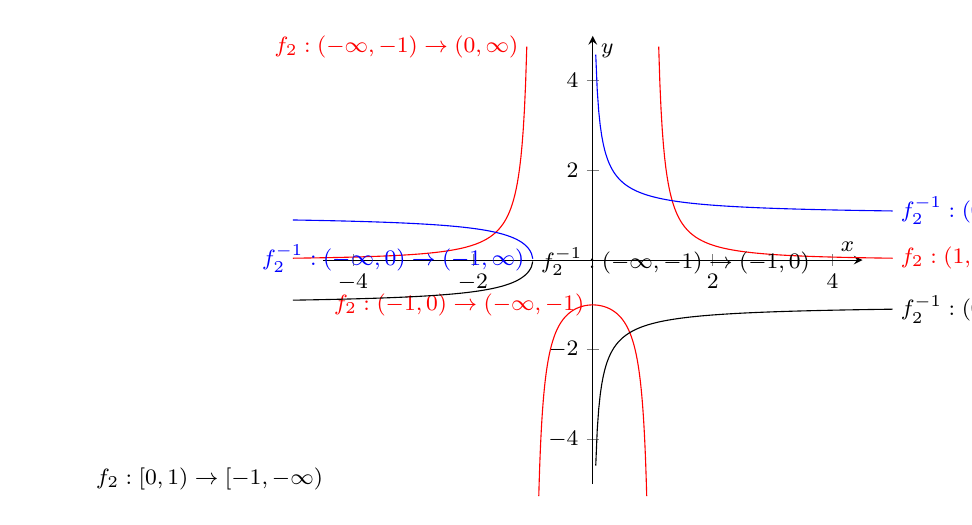
\begin{tikzpicture}
    \begin{axis}[
     axis lines=middle,clip=false,
            xmin=-4.5,xmax=4.5, ymin=-5,ymax=5,
            xticklabel style={black},
            xlabel=$x$,
            ylabel=$y$]
    \addplot[domain=-5:-1.1,samples=200,red]{1/(x^2-1)}
    node[left,pos=1.,font=\footnotesize]{$f_2:(-\infty, -1) \to (0,\infty)$};
    \addplot[domain=-0.9:0,samples=200,red]{1/(x^2-1)}
    node[left,pos=1.,font=\footnotesize]{$f_2:(-1,0) \to (-\infty, -1)$};
    \addplot[domain=0:0.9,samples=200,red]{1/(x^2-1)};
    node[left,pos=1.,font=\footnotesize]{$f_2:[0,1) \to [-1,-\infty)$};
    \addplot[domain=1.1:5,samples=200,red]{1/(x^2-1)}
    node[right,pos=1.,font=\footnotesize]{$f_2:(1,\infty) \to (0,\infty)$};
    \addplot[domain=-5:-1.001,samples=200,blue]{sqrt((1+x)/x)}
    node[left,pos=1.,font=\footnotesize]{$f_2^{-1}:(-\infty,0) \to (-1,\infty)$};
    \addplot[domain=0.05:5,samples=200,blue]{sqrt((1+x)/x)}
    node[right,pos=1.,font=\footnotesize]{$f_2^{-1}:(0,\infty) \to (1,\infty)$};
    \addplot[domain=-5:-1.001,samples=200,black]{-sqrt((1+x)/x)}
    node[right,pos=1.,font=\footnotesize]{$f_2^{-1}:(-\infty,-1) \to (-1,0)$};
    \addplot[domain=0.05:5,samples=200,black]{-sqrt((1+x)/x)}
    node[right,pos=1.,font=\footnotesize]{$f_2^{-1}: (0,\infty) \to (-\infty,-1)$};
    \end{axis}
\end{tikzpicture}
\newpage

\item
Die Funktion $\arcsin(x)$ ist die Umkehrfunktion von $\sin(x)$, wenn nur der Hauptwert betrachtet wird.
Nach Definition, schr\"anken wir den Definitionsbereich von $\sin(x)$ ein auf $-\frac{\pi}{2} \leq x \leq \frac{\pi}{2}$, 
w\"ahrend der Wertebereich $[-1,1]$ ist.
Die erste Ableitung von $\sin(x)$ ist $\cos(x) \geq 0$ f\"ur alle $x \in [-\frac{\pi}{2},\frac{\pi}{2}]$,
daher ist die Funktion monoton steigend und folglich injektiv.
Als Abbildung $f_3 : [-\frac{\pi}{2},\frac{\pi}{2}] \to [-1,1]$ ist die Funktion bijektiv.
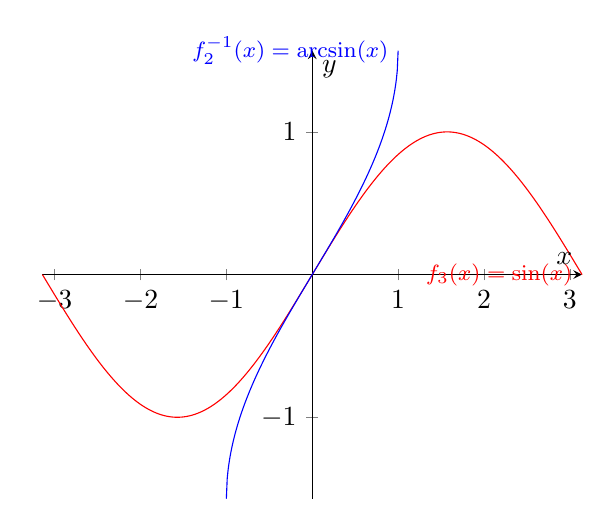
\begin{tikzpicture}
    \begin{axis}[
     axis lines=middle,clip=false,
            xmin=-pi,xmax=pi, ymin=-pi/2,ymax=pi/2,
            xticklabel style={black},
            xlabel=$x$,
            ylabel=$y$]
    \addplot[domain=-pi:pi,samples=200,red]{sin(deg(x))}
    node[left,pos=1.,font=\footnotesize]{$f_3(x)=\sin(x)$};
    \addplot[domain=-1:1,samples=200,blue]{asin(x)/180*pi}
    node[left,pos=1.,font=\footnotesize]{$f_2^{-1}(x)=\arcsin(x)$};
    \end{axis}
\end{tikzpicture}
\newpage
\item
Die Funktion $\arctan(x)$ ist die Umkehrfunktion von $\tan(x)$, wenn nur der Hauptwert betrachtet wird. 
Nach Definition beschr\"anken wir den Definitionsbereich von $\tan(x)$ auf $-\frac{\pi}{2}< x <\frac{\pi}{2}$, 
w\"ahrend der Wertebereich $(-\infty,\infty)$ ist.
Die erste Ableitung von $\tan(x)$ ist $\frac{1}{\cos^2(x)} > 0$ f\"ur alle $x \in (-\frac{\pi}{2},\frac{\pi}{2})$, daher ist die Funktion 
monoton steigend und folglich injektiv. 
Als Abbildung $f_3 : (-\frac{\pi}{2},\frac{\pi}{2}) \to (-\infty,\infty)$ ist sie bijektiv
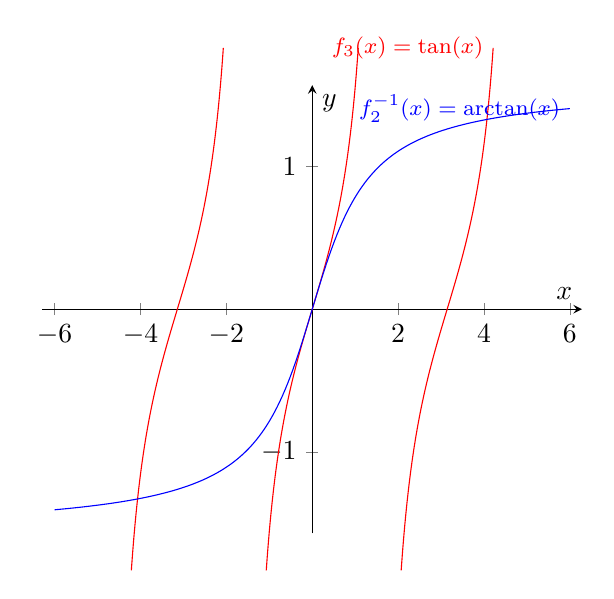
\begin{tikzpicture}
    \begin{axis}[
     axis lines=middle,clip=false,
            xmin=-2*pi,xmax=2*pi, ymin=-pi/2,ymax=pi/2,
            xticklabel style={black},
            xlabel=$x$,
            ylabel=$y$]
    \addplot[domain=-pi/2+0.5:pi/2-0.5,samples=200,red]{tan(deg(x))};
    \addplot[domain=-3*pi/2+0.5:-pi/2-0.5,samples=200,red]{tan(deg(x))};
    \addplot[domain=pi/2+0.5:3*pi/2-0.5,samples=200,red]{tan(deg(x))}
    node[left,pos=1.,font=\footnotesize]{$f_3(x)=\tan(x)$};
    \addplot[domain=-6:6,samples=200,blue]{atan(x)/180*pi}
    node[left,pos=1.,font=\footnotesize]{$f_2^{-1}(x)=\arctan(x)$};
    \end{axis}
\end{tikzpicture}
%clear all
%close all
%
%f=@(x) exp(1./x)
%
%% plot function and inverse branches
%
%% pt. I
%a=-3; b=-.01;
%
%x=linspace(a,b,100)';
%y=f(x);
%
%figure, plot(x,y,'LineWidth',2), hold on, grid, plot(y,x,'LineWidth',2), axis equal
%
%% pt. II
%a=.8; b=3.5;
%
%x=linspace(a,b,100)';
%y=f(x);
%
%figure, plot(x,y,'LineWidth',2), hold on, grid, plot(y,x,'LineWidth',2), axis equal

%clear all
%close all
%
%f=@(x) 1./(x.*x-1)
%
%% plot function and inverse branches
%
%% pt. I
%a=-10; b=-1.1;
%
%x=linspace(a,b,100)';
%y=f(x);
%
%figure, plot(x,y,'LineWidth',2), hold on, grid, plot(y,x,'LineWidth',2), axis equal
%
%% pt. II
%a=-.9; b=-.01;
%
%x=linspace(a,b,100)';
%y=f(x);
%
%figure, plot(x,y,'LineWidth',2), hold on, grid, plot(y,x,'LineWidth',2), axis equal
%
%% pt. III
%a=0; b=.9;
%
%x=linspace(a,b,100)';
%y=f(x);
%
%figure, plot(x,y,'LineWidth',2), hold on, grid, plot(y,x,'LineWidth',2), axis equal
%
%% pt. IV
%a=1.1; b=10;
%
%x=linspace(a,b,100)';
%y=f(x);
%
%figure, plot(x,y,'LineWidth',2), hold on, grid, plot(y,x,'LineWidth',2), axis equal

\end{iii}
}



\ifthenelse{\boolean{mitLoes}}{\ruleBig \cleardoublepage}{}
% 59
\Aufgabe[e]{Kurvendiskussion}{\label{KurvDisk002}

Gegeben sei die Funktion
$$	f(x) = \dfrac{x^2+3\,x}{1-x}.$$
\begin{iii}
	\item Geben Sie den maximalen Definitionsbereich der Funktion \ $f$ \ an.
	
	\item Bestimmen Sie die Nullstellen der Funktion.
	
	\item Bestimmen Sie die kritischen Punkte der Funktion und deren Funktionswerte. Klassifizieren Sie alle kritischen Punkte als Minimum, Maximum oder Wendepunkt.
	
	\item Untersuchen Sie das Monotonieverhalten der Funktion. 
	
	\item Bestimmen Sie alle Asymptoten der Funktion.

	\item Bestimmen Sie den Wertebereich der Funktion.

	\item Skizzieren Sie die Funktion.
\end{iii}
}

\Loesung{
\begin{abc}
\item
\begin{iii}
	\item Der maximale Definitionsbereich ist \ $\mathcal D = \R\backslash\left\{1\right\}$\,.
	
	\item Die Nullstellen der Funktion sind \ $x_{N_1} = -3 \text{ und } x_{N_2} = 0$ \,.
	
	\item Die kritischen Punkte sind die Nullstellen der ersten Ableitung. Aus
$$	f'(x) = \frac{(2x+3)(1-x)+(x^2+3x)}{(1-x)^2} = \dfrac{-x^2+2\,x+3}{(1-x)^2}=0  $$
  folgt
$$
  x_{K_1}= -1\text{ mit } f(-1)=-1 \text{ und } x_{K_2}= 3\text{ mit } f(3)=-9\ .
$$
  	Die zweite Ableitung ist:
  	$$
		f''(x) = \frac{8}{(1-x)^3}.
  	$$
  	Für $x_{K_1}= -1$ ist $f''(-1)=1 > 0$. Es handelt sich also um ein Minimum.
  	Für $x_{K_2}= 3$ ist $f''(3)=-1 < 0$. Es handelt sich also um ein Maximum.
  	
	\item
	Aus den stationären Punkten un der Definitionslücke ergeben sich die Monotonieintervalle.
	In $(-\infty, -1)$ und $(3,\infty)$ ist die Funktion monoton fallend. In $(-1,1)$ und 
	$(1,3)$ ist die Funktion monoton steigend. 
	\item Aus  $f(x) = -x-4+\dfrac{4}{1-x}$  folgt, dass  $g(x)=-x-4$  die Asymptote ist.
	Wegen $\lim_{x \to 1^-} f(x) = \infty$ und $\lim_{x \to 1^+} f(x) = -\infty$ gibt es 
	eine senkrechte Asymptote bei $x=1$.
	\item Der Wertebereich ist $\mathcal{W} = (-\infty,-9] \cup [-1,\infty)$. 
	\item \quad\\
\end{iii}
\end{abc}
\begin{center}	
\psset{unit=0.5cm}
\begin{pspicture}(-5,-16)(7,6)

\psgrid[griddots=8,subgriddiv=0](-5,-16)(7,6)
\psline[linestyle=dashed](-5,1)(7,-11)
\psline[linestyle=dashed](1,-16)(1,6)

\pscircle*(-3,0){0.1}
\pscircle*(-1,-1){0.1}
\pscircle*(-0,0){0.1}
\pscircle*(3,-9){0.1}
\psplot[plotpoints=100, plotstyle=curve]
{-5}{.63}
{
x x mul 3 x mul add 1 x neg add div
}
\psplot[plotpoints=100, plotstyle=curve]
{1.37}{7}
{
x x mul 3 x mul add 1 x neg add div
}

\end{pspicture}

\end{center}

Bei \ $(-1,-1)$ \ handelt es sich also um ein (lokales) Minimum, bei \ $(3,-9)$ \ um ein Maximum.
}

\ErgebnisC{AufganalysKurvDisk002}
{
\textbf{a)}\textbf{ii)} $0,\, -3$, 
\textbf{iii)} -1,\, 3, 
\textbf{iv)} $g(x)=-x-4$
}

\ifthenelse{\boolean{mitLoes}}{\ruleBig \cleardoublepage}{}
% 115
\Aufgabe[e]{Stationäre Punkte}{
Gegeben sei die Funktion
$$	g\,:\,\R\rightarrow\R\,:\,x\rightarrow \big(x^2-4\big)^2\cdot\EH{-x} .$$
Bestimmen Sie alle relativen Minima und Maxima der Funktion \ $g$ \ \textbf{ohne} 
die zweite Ableitung zu berechnen.
}


\Loesung{

Da die Funktion nirgends negativ ist, sind die Nullstellen automatisch lokale Minima: 
\ $x_{\text {min}_{1,2}} = \pm 2$\,. 

Die Nullstellen der ersten Ableitung sind die kritischen Punkte. Aus
$$
	g'(x) = 4x\,(x^2-4)\,\EH{-x}-(x^2-4)^2\,\EH{-x} = (-x^2+4x+4)(x^2-4)\,\EH{-x}=0  
$$
folgt
$$
	x_{1,2} =\pm 2 \text{ und } x_{3,4} = 2\pm\sqrt 8.
$$
Die ersten beiden kritischen Punkte sind die schon bekannten Nullstellen und die 
beiden anderen sind
Maxima, da ein einfacher kritischer Punkt zwischen zwei Minima nur ein Maximum sein 
kann und die
Funktion für \ $x\rightarrow\infty$ \ gegen \ 0 \ geht.

}

\ErgebnisC{StationaerePunkte}
{
$x_{\text {min}} = \pm 2$,  $x_{\text{max}} = 2\pm\sqrt 8$
}

\ifthenelse{\boolean{mitLoes}}{\ruleBig \cleardoublepage}{}
% 58
\Aufgabe[e]{Kurvendiskussion}{
Bestimmen Sie den maximalen Definitionsbereich, die Symmetrie, alle Nullstellen, sowie Art und Lage
der kritischen Punkte und Wendepunkte der rellen Funktion
$$  f(x) =x \sqrt{16-x^2}.$$

}

\Loesung{
\begin{iii}
\item Der maximale Definitionsbereich ist \ $D = [-4,4]$ .
\item Die Funktion \ $f$ \ ist ungerade bzw. punktsymmetrisch zum Ursprung:
$$
  f(x) = x\sqrt{16-x^2} = -(-x)\sqrt{16-(-x)^2}=-f(-x)\ .
$$
\item  Die Nullstellen sind 
\begin{align*}
&&0=& x \sqrt{16-x^2}\\
\Leftrightarrow&&x=&0\,\text{ oder }\, 16=x^2\\
\Leftrightarrow&&x\in& \{0,\, 4,\, -4\}
\end{align*}
\item Kritische Punkte liegen bei $x\in D$ mit: 
\begin{align*}
&&0=& f'(x) = \sqrt{16-x^2}-\frac{x\cdot x}{\sqrt{16-x^2}}=\frac{16-2x^2}{\sqrt{16-x^2}}\\
\Leftrightarrow &&\pm 4 =& \sqrt 2 x \quad\Leftrightarrow \quad x=\pm 2\sqrt{2}
\end{align*}
Die Funktion $f$ selbst hat an den Grenzen des Definitionsbereiches $D$ sowie im Ursprung den Wert
$f(0)=f(\pm 4)=0$ 
F\"ur alle anderen $x>0$ ist $f(x)>0$. Also muss im Punkt $x=+2\sqrt 2$ das absolute (und damit auch
ein relatives) Maximum $f(2\sqrt 2)=8$ der Funktion liegen. \\
Mit der Symmetrie der Funktion folgt, dass in $x=-2\sqrt 2$ ein Minimum $f(-2\sqrt 2)=-8$ liegt. 
\item  Wendepunkte und Konvexität:\\
Zun\"achst ist 
\begin{align*}
f''(x)=& \frac{-4x\sqrt{16-x^2}-(16-2x^2)\cdot (-2x)\frac 12(16-x^2)^{-1/2}}{16-x^2}\\
=& \frac{-4x(16-x^2)+x(16-2x^2)}{(16-x^2)^{3/2} }\\
=& \frac{2x^3-48x}{(16-x^2)^{3/2}}
\end{align*}
Die einzige reelle Nullstelle des Z\"ahlers im Definitionsbereich $]-4,4[$ ist $x=0$ und es gilt
$$
   f''(x)=	\begin{cases}
					>0 & \text{für }x \in ]-4,0[\\
					<0 & \text{für }x \in ]0,4[ 
				\end{cases}
$$
Also liegt in $(0,0)$ ein Wendepunkt, links davon ist $f$ konvex und rechts davon konkav. \\

\unitlength1cm
\begin{picture}(2.5,9)
\put(5.5,4){\begin{picture}(0,0)\unitlength1cm
\thinlines
\put( -4.5,0){\vector(1,0){10}}
\multiput( -4 , -0.1)(1,0){9}{\line(0,1){0.2}}
\put(.9,-0.4){{ 1}}
\put( 0,-4.25){\vector(0,1){8.75}}
\multiput( -0.1,-4)(0,1){9}{\line(1,0){0.2}}
\put(-0.5,.9){{ 2}}

\thicklines
\bezier{200}( -4.000, -0.002)( -4.000, -2.748)( -3.333, -3.685)
\bezier{200}( -3.333, -3.685)( -3.047, -4.089)( -2.667, -3.975)
\bezier{200}( -2.667, -3.975)( -2.365, -3.885)( -2.000, -3.464)
\bezier{200}( -2.000, -3.464)( -1.697, -3.114)( -1.333, -2.514)
\bezier{200}( -1.333, -2.514)( -1.041, -2.032)( -0.667, -1.315)
\bezier{200}( -0.667, -1.315)( -0.445, -0.891)(  0.000,  0.000)
\bezier{200}(  0.000,  0.000)(  0.445,  0.891)(  0.667,  1.315)
\bezier{200}(  0.667,  1.315)(  1.041,  2.032)(  1.333,  2.514)
\bezier{200}(  1.333,  2.514)(  1.697,  3.114)(  2.000,  3.464)
\bezier{200}(  2.000,  3.464)(  2.365,  3.885)(  2.667,  3.975)
\bezier{200}(  2.667,  3.975)(  3.047,  4.089)(  3.333,  3.685)
\bezier{200}(  3.333,  3.685)(  4.000,  2.748)(  4.000,  0.002)

\end{picture}}
\end{picture}

\end{iii}
}

\ErgebnisC{AufganalysKurvDisk001}
{
$D(f)= [-4,4]$, $f$ ist ungerade, Nullstellen: $x=0,\pm 4$, Extrema bei $x=\pm 2\sqrt 2$, \\
Wendepunkt
bei $x=0$

}

\ifthenelse{\boolean{mitLoes}}{\ruleBig \cleardoublepage}{}

%\Aufgabe[e]{}
{

Gegeben sei die Funktion $f(x) = \cos \left(\dfrac{\pi}{2} \sin x\right)$.

\begin{iii}
 
 \item Bestimmen Sie den Definitionsbereich und den Wertebereich von $f$. 
 
 \item Zeigen Sie, dass die Funktion $f$ die Periodizität $\pi$ besitzt, d.h.\ zeigen Sie, dass $f(x+\pi) = f(x)$ für alle $x\in \R$ gilt.
 
 \item Bestimmen Sie alle Nullstellen von $f$.\\[0.5ex]
 \textbf{Hinweis:} Beachten Sie die Periodizität von $f$.
 
 \item Bestimmen Sie alle Extrema von $f$ und charakterisieren Sie diese.\\[0.5ex]
 \textbf{Hinweis:} Beachten Sie die Periodizität von $f$.
 
 \item Skizzieren Sie den Graphen von $f$ im Intervall $[-\pi,2\pi]$. 
 
\end{iii}
}


\Loesung{
\begin{iii}
\item  Der Wertebereich der Sinusfunktion ist $[-1,1]$. Auf $[-\pi/2,\pi/2]$ 
nimmt der Kosinus alle Werte von $0$ bis $1$ an. Somit gilt 
\[
D(f) =\R \qquad \text{ und } \qquad W(f) = [0,1]\,.
\]

\medskip
\item  Es gilt
\begin{align*}
 f(x+\pi) &  = \cos \left(\frac{\pi}{2} \sin (x+\pi)\right)\\[1ex]
 & = \cos \left(-\frac{\pi}{2} \sin x \right)\\[1ex]
 & = \cos \left(\frac{\pi}{2} \sin x\right)\\[1ex]
 & = f(x) 
\end{align*}
für alle $x\in \R$. Somit hat $f$ die Periode $\pi$. Hinweis: Es lässt sich zeigen, dass $f$ keine kleinere Periode als $\pi$ besitzt. 

\medskip
\item Aufgrund der Periodizität reicht es aus, die Nullstellen im Intervall $[0,\pi]$ zu bestimmen. Es gilt 
\begin{align*}
 f(x) & = \cos \left(\frac{\pi}{2} \sin x\right) = 0 \\[1ex]
 \Longleftrightarrow \quad \frac{\pi}{2} \sin x & = \frac{\pi}{2}\,.
\end{align*}
Es ergibt sich $x=\pi/2$. Die Menge aller Nullstellen ist somit
\[
N = \left\{\frac{\pi}{2} + k\pi \;\; \Big| \;\; k\in \mathbb Z \right\}\,.
\]

\medskip
\item Es gilt 
\[
f'(x) = - \sin \left(\frac{\pi}{2}\sin x\right)\frac{\pi}{2}\cos x\,.
\]
Es folgt 
\begin{align*}
 f'(x) & = - \sin \left(\frac{\pi}{2}\sin x\right)\frac{\pi}{2}\cos x = 0 \\[1ex]
 \Longleftrightarrow \quad \sin \left(\frac{\pi}{2}\sin x\right) & = 0 \quad \text{oder} \quad \cos x = 0\,.
\end{align*}
Der erste Fall liefert $x=0$ und $x=\pi$. Der zweite Fall ergibt $x=\pi/2$. Da $f$ nur Werte zwischen $0$ und $1$ annimmt, sind $x_1=(0,1)$ und $x_3=(\pi,1)$ Maxima, während $x_2 = (\pi/2,0)$ Minimum ist. Die Menge aller Maxima ist 
\[
E_{\max} = \{(k\pi,1) \mid k\in \mathbb Z \}\,.
\]
Die Menge aller Minima ist
\[
E_{\max} = \left\{ \left(\frac{\pi}{2}+k\pi,0\right) \mid k\in \mathbb Z \right\}\,.
\]

\medskip
\item
\end{iii}
\begin{center}
	\begin{pspicture}(-4,-1)(7,2)
	\psgrid[griddots=8,subgriddiv=0](-4,-1)(7,2)
	\psline[linewidth=1.2pt]{->}(-4,0)(7,0)
	\psline[linewidth=1.2pt]{->}(0,-1)(0,2)
        \psplot[plotpoints=100, plotstyle=curve]{-4}{7}
        {
        x 180 mul 3.14159 div sin 90 mul cos
        }
        \psdot(-1.5708,0)
        \psdot(1.5708,0)
        \psdot(4.7124,0)
        \psdot(  -3.14159,   1.00000)
        \psdot(   0.00000,   1.00000)
        \psdot(   3.14159,   1.00000)
        \psdot(   6.283  ,   1.00000)
        \psdot(  -1.57080,   0.00000)
        \psdot(   1.57080,   0.00000)
        \psdot(   4.71239,   0.00000)

%\cos \left(\dfrac{\pi}{2} \sin x\right)$.



	\end{pspicture} 

%\boxed{\includegraphics[width =0.25\textwidth]{./fig_f.eps}}
\end{center}

}


%\ifthenelse{\boolean{mitLoes}}{\ruleBig \cleardoublepage}{}
%% 60
%\Aufgabe[e]{Kurvendiskussion}{
F\"uhren Sie eine Kurvendiskussion f\"ur die Funktion 
$$f(x)=\ln (3x^2+2x+1)$$
durch. Bestimmen Sie dazu: 
\begin{abc}
\item den maximalen Definitionsbereich von $f$, 
\item die Symmetrieachsen von $f$, d. h. Werte $\alpha\in \R$, so dass $f(\alpha+x)=f(\alpha-x)$, 
\item das Verhalten von $f$ im Unendlichen, 
\item die Nullstellen von $f$, 
\item die Extrema und das Monotonieverhalten von $f$, 
\item sowie die Wendepunkte und das Kr\"ummungsverhalten von $f$. 
\item Skizzieren Sie den Graphen von $f$. 
\end{abc}
}

\Loesung{
\begin{abc}
\item Die Funktion ist f\"ur alle $x\in \R$ definiert, weil das Argument der Logarithmusfunktion
immer positiv ist: 
$$3x^2+2x+1=\left(\sqrt 3 x+ \frac 1{\sqrt 3}\right)^2 +1-\frac 13>1-\frac 13>0.$$
\item Gesucht ist ein $\alpha\in \R$, so dass f\"ur alle $x\in \R$ gilt: 
\begin{align*}
&& f(\alpha+x)=& f(\alpha-x)\\
\Leftrightarrow&& \ln (3(\alpha+x)^2+2(\alpha+x)+1)=& \ln (3(\alpha-x)^2+2(\alpha-x)+1)\\
\Leftrightarrow&& 3(\alpha+x)^2+2(\alpha+x)+1=& 3(\alpha-x)^2+2(\alpha-x)+1&\text{ (Monotonie
von $\ln$)}\\
\Leftrightarrow&&6x\alpha+2x=&-6x\alpha-2x\\
\Leftrightarrow&&(12\alpha+4)x=&0\\
\Leftrightarrow&&12\alpha+4=& 0
\end{align*}
Also liegt die Symmetrieachse bei $\alpha=-1/3$. 
\item Es ist 
$$\underset{x\to \pm\infty}\lim f(x)=\infty.$$
\item Die einzige Nullstelle des Logarithmus liegt bei $1$, also muss f\"ur $f(x)=0$ gelten:
$$1=3x^2+2x+1\Rightarrow x\in\{0,-2/3\}.$$
\item Die Nullstellen der Ableitung berechnen sich zu: 
\begin{align*}
0=& f'(x)= \frac 1{3x^2+2x+1}\cdot (6x+2)\,\Rightarrow \, x=-\frac 13.
\end{align*}
Dies ist die einzige Nullstelle der Ableitung. Da die Funktion bez\"uglich dieser Achse symmetrisch
ist, und f\"ur $x\rightarrow \pm \infty$ gegen $\infty$ geht, liegt bei $x=-1/3$ ein Minimum. 
\item Die Wendepunkte liegen an den Nullstellen der zweiten Ableitung:
\begin{align*}
&&0=& f''(x)=\frac{6(3x^2+2x+1)-(6x+2)^2}{(3x^2+2x+1)^2}=\frac{-18x^2-12x+2}{(3x^2+2x+1)^2}\\
\Rightarrow&&x=&\frac{-1\pm \sqrt 2}3.
\end{align*}
Links von $-1/3-\sqrt{2}/3$ ist $f''(x)<0$, also ist die Funktion dort konkav, rechts von
$-1/3-\sqrt 2/3 $ ist $f''(x)>0$
und die Funktion $f$ ist dort konvex. Rechts von $-1/3+\sqrt 2/3$ ist die Funktion wegen der
Symmetrie wiederum konkav. 
\item \quad\\
\begin{minipage}{.4\textwidth}
\psset{xunit=1.8cm, yunit=1.8cm, runit=1cm}
\begin{pspicture}(-3,-1)(2,3)
\psgrid[subgriddiv=1,griddots=10,gridlabels=.3](-3,-1)(2,3)
\psline{-}(-.333,-1)(-.333,3)
\psplot[plotpoints=200, plotstyle=curve]
{-2.333}{2}
{3 x mul x mul 2 x mul add 1 add ln}
\psdot(0,0)
\psdot(-.666,0)
\psdot(-.333,-.405)
\psdot(.138,.288)
\psdot(-.805,.288)
\end{pspicture}
\end{minipage}
\end{abc}
}

\ErgebnisC{AufganalysKurvDisk004}
{
{\textbf{ b)}} $\alpha=-1/3$,
{\textbf{ d)}} $0$, $-2/3$,
{\textbf{ e)}} Minimum bei $-1/3$,
{\textbf{ f)}} Wendepunkte bei $-1/3\pm \sqrt 2/3$
}

%\ifthenelse{\boolean{mitLoes}}{\ruleBig \cleardoublepage}{}
%\Aufgabe[e]{Grenzwert}
{
Bestimmen Sie den Grenzwert 
\[
\lim_{x\rightarrow \infty} (x+3)\left(\operatorname e^{2/x}-1\right)\,.
\]

}

\Loesung{
 Es gilt 
\[
(x+3)\left(\operatorname e^{2/x}-1\right) = \frac{\operatorname 
e^{2/x}-1}{\dfrac{1}{x+3}} =: \frac{f(x)}{g(x)}
\]
mit $\lim_{x\rightarrow \infty} f(x) = 0$ und $\lim_{x\rightarrow \infty} g(x) = 0$. Mit 
dem Satz von L'Hospital folgt dann
\begin{align*}
 \lim_{x\rightarrow \infty} \dfrac{f(x)}{g(x)} & = \lim_{x\rightarrow \infty }
\dfrac{f'(x)}{g'(x)} = \lim_{x\rightarrow \infty} \dfrac{2\operatorname e^{2/x} 
(x+3)^2}{x^2} \\[1ex]
& = \lim_{x\rightarrow \infty} 2\operatorname e^{2/x} \, \lim_{x\rightarrow \infty} 
\dfrac{(x+3)^2}{x^2} = 2\,.
\end{align*}
}

%\ifthenelse{\boolean{mitLoes}}{\ruleBig \cleardoublepage}{}

%\Aufgabe[e]{Stationäre Punkte}{
Gegeben sei die Funktion
$$	g\,:\,\R\rightarrow\R\,:\,x\rightarrow \big(x^2-4\big)^2\cdot\EH{-x} .$$
Bestimmen Sie alle relativen Minima und Maxima der Funktion \ $g$ \ \textbf{ohne} 
die zweite Ableitung zu berechnen.
}


\Loesung{

Da die Funktion nirgends negativ ist, sind die Nullstellen automatisch lokale Minima: 
\ $x_{\text {min}_{1,2}} = \pm 2$\,. 

Die Nullstellen der ersten Ableitung sind die kritischen Punkte. Aus
$$
	g'(x) = 4x\,(x^2-4)\,\EH{-x}-(x^2-4)^2\,\EH{-x} = (-x^2+4x+4)(x^2-4)\,\EH{-x}=0  
$$
folgt
$$
	x_{1,2} =\pm 2 \text{ und } x_{3,4} = 2\pm\sqrt 8.
$$
Die ersten beiden kritischen Punkte sind die schon bekannten Nullstellen und die 
beiden anderen sind
Maxima, da ein einfacher kritischer Punkt zwischen zwei Minima nur ein Maximum sein 
kann und die
Funktion für \ $x\rightarrow\infty$ \ gegen \ 0 \ geht.

}

\ErgebnisC{StationaerePunkte}
{
$x_{\text {min}} = \pm 2$,  $x_{\text{max}} = 2\pm\sqrt 8$
}

%\ifthenelse{\boolean{mitLoes}}{\ruleBig \cleardoublepage}{}






% \ifthenelse{\boolean{mitLoes}}{\cleardoublepage}{}
\ifthenelse{\boolean{mitErg}}{
\ruleBig
\Ergebnisse}{}


\end{twocolumn}
\end{document}
